% Author: Izaak Neutelings (July 2017)
% Timelines & energy scales of particle physics
\documentclass[border=1pt,tikz]{standalone}

\usepackage{amsmath} % for \dfrac
\usepackage{tikz}
\tikzset{>=latex} % for LaTeX arrow head

\begin{document}

% LOGARITHMIC SCALE
\large
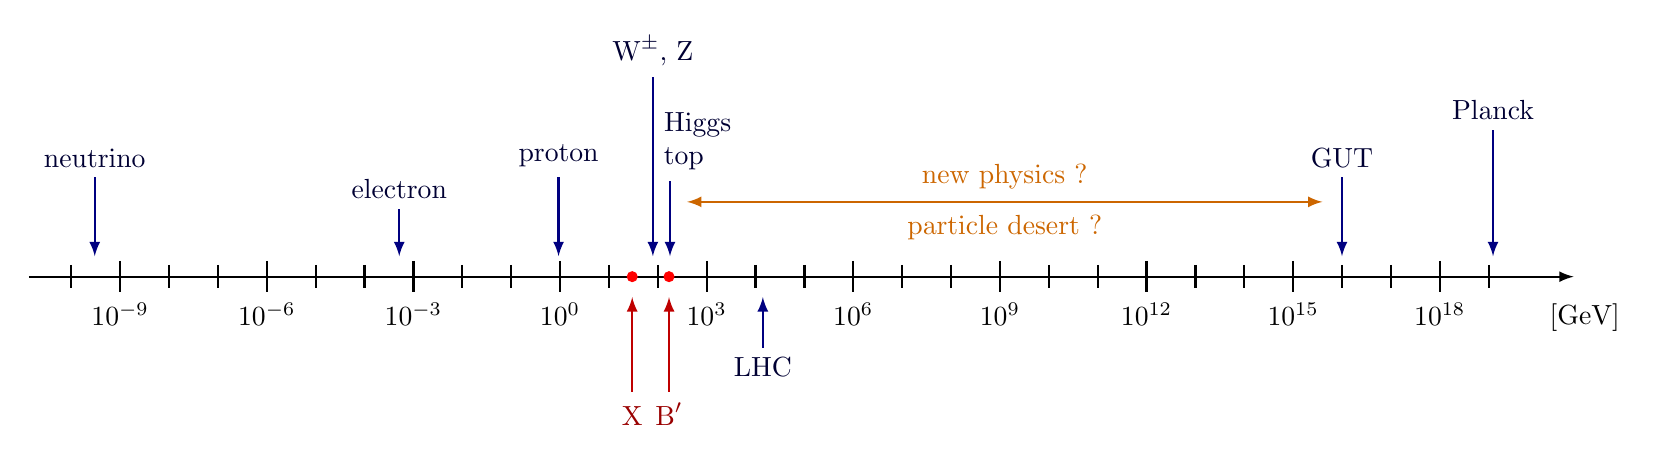
\begin{tikzpicture}[]
  
  % limits
  \newcount\nOne; \nOne=-10
  \def\w{18}      % width of axes
  \def\n{29}      % number of decades
  \def\noffset{1} % offset labels
  \def\nskip{3}   % skip number
  \def\la{2.00}   % arrow length
  \def\lt{0.20}   % tick length
  \def\ls{0.15}   % tick length (skipped)
  
  % help functions
  \def\myx(#1){{(#1-\nOne)*\w/\n}}
  \def\arrowLabel(#1,#2,#3,#4){
    \def\xy{(#1-\nOne)*\w/\n}; \pgfmathparse{int(#2*100)};
    \ifnum \pgfmathresult<0
      \def\yyp{{(\lt*(-0.10+#2))}}; \def\yyw{{(\yyp-\la*\lt*#3)}}
      \draw[<-,thick,black!50!blue,align=center]
        (\myx(#1),\yyp) -- (\myx(#1),\yyw)
        node[below,black!80!blue] {#4}; %,fill=white
    \else
      \def\yyp{{(\lt*(0.10+#2)}}; \def\yyw{{(\yyp+\la*\lt*#3)}}
      \draw[<-,thick,black!50!blue,align=center]
        (\myx(#1),\yyp) -- (\myx(#1),\yyw)
        node[above,black!80!blue] {#4};
    \fi}
  \def\arrowLabelRed(#1,#2,#3,#4){
    \def\yyp{{(\lt*(-0.10+#2))}}; \def\yyw{{(\yyp-\la*\lt*#3)}}
    \fill[red,radius=2pt] (\myx(#1),0) circle;
    \draw[<-,thick,black!25!red,align=center]
      (\myx(#1),\yyp) -- (\myx(#1),\yyw)
      node[below,black!40!red] {\strut#4}; %,fill=white
    }
  
  % axis
  \draw[->,thick] (-\w*0.03,0) -- (\w*1.06,0)
                  node[right=4pt,below=6pt] {[GeV]};
  
  % ticks
  \foreach \tick in {0,1,...,\n}{
    \def\x{{\tick*\w/\n}}
    \def\dec{\the\numexpr \nOne+\tick \relax}
	\pgfmathparse{Mod(\tick-\noffset,\nskip)==0?1:0}
	\ifnum\pgfmathresult>0
	  \draw[thick] (\x,\lt) -- (\x,-\lt) % ten tick
	               node[below] {$10^{\dec}$}; % label
	\else
      \draw[thick] (\x,\ls) -- (\x,-\ls); % ten tick
	\fi
  }
  
  % label
  \arrowLabel(-9.52,1.2,2.5,neutrino) % log(0.0000000003)=-9.523 (0.3 eV)
  \arrowLabel(-3.29,1.2,1.5,electron) % log(0.000510)=-3.292 (0.510 MeV)
  \arrowLabel(-0.03,1.2,2.5,proton)   % log(0.938)=-0.03
  \arrowLabel( 1.90,1.2,5.7,$\text{W}^\pm$, $\text{Z}$) % log(80)=1.90, log(90)=1.95
  \arrowLabel( 2.25,1.2,2.4,\qquad Higgs\\\quad top) % log(125)=2.10, log(175)=2.24
  \arrowLabel( 4.15,-1.2,1.6,LHC)     % log(1400)=4.146
  \arrowLabel(16.00,1.2,2.5,GUT)      % 10^25 eV = 10^16 GeV
  \arrowLabel(19.09,1.2,4.0,Planck)   % Planck % quantum gravity % 1.22x10^19 . GeV
  
  % low mass
  \arrowLabelRed(1.477,-1.2,3.0,X)    % ln(30) = 1.477
  \arrowLabelRed(2.230,-1.2,3.0,$\text{B}'$) % ln(170) = 2.230
  
  % stretch
  \draw[<->,thick,black!20!orange]
    ({(2.6-\nOne)*\w/\n},0.95) -- ({(15.6-\nOne)*\w/\n},0.95)
    node[midway,below=1pt] {particle desert ?}
    node[midway,above=1pt] {new physics ?};
  
\end{tikzpicture}




\end{document}